% ─────────────────────────────────────────────────────────────────
\section{Results and Comparison}
\label{sec:results}
% ─────────────────────────────────────────────────────────────────

\subsection{Main Results Table}

Table~\ref{tab:main_results} summarises all runs in this study alongside
two external SHREC\,25 entries.
All HierGIN metrics use the proper 88-class evaluation protocol
(Section~\ref{sec:eval_protocol}); external numbers are as published
in the SHREC\,25 challenge report~\cite{shrec25}.

\begin{table}[ht]
  \centering
  \caption{Test set performance --- all runs (88-class evaluation).
           \textbf{Bold}: best value per metric column.
           $\dagger$~RI-GIN 14D is running at the time of writing.
           $\ddagger$~Injection runs use 14D (global norm) features as base.
           External method metrics are as published.}
  \label{tab:main_results}
  \setlength{\tabcolsep}{4.5pt}
  \begin{tabular}{llrrrr}
    \toprule
    \textbf{Method} & \textbf{Features}
      & \textbf{Acc} & \textbf{Bal.Acc} & \textbf{Macro-F1} & \textbf{Wtd-F1} \\
    \midrule
    \multicolumn{6}{l}{\textit{External baselines}} \\
    \quad Flat GIN (h512, 6L)         & 4D          & ---   & ---   & 0.640 & ---   \\
    \quad Mamba3D~\cite{mamba3d}      & point cloud & ---   & 0.662 & 0.672 & 0.825 \\
    \quad PointMamba~\cite{pointmamba}& point cloud & ---   & 0.714 & 0.720 & 0.872 \\
    \midrule
    \multicolumn{6}{l}{\textit{HierGIN --- feature ablation (standard GIN backbone)}} \\
    \quad HierGIN 6D                  & xyz + normals        & 0.783 & 0.612 & 0.619 & 0.760 \\
    \quad HierGIN 7D (no Pot)         & no Potential         & 0.808 & 0.681 & 0.680 & 0.799 \\
    \quad HierGIN 4D                  & xyz + Potential      & 0.845 & 0.796 & 0.784 & 0.843 \\
    \quad HierGIN 7D (no NormPot)     & no NormalPotential   & 0.849 & 0.797 & 0.790 & 0.848 \\
    \quad HierGIN 8D                  & all 8 features       & 0.853 & 0.800 & 0.798 & 0.853 \\
    \midrule
    \multicolumn{6}{l}{\textit{HierGIN --- enriched features (14D = 8D + 6 geometric)}} \\
    \quad HierGIN 14D (z-scored)      & per-protein z-score  & 0.838 & 0.757 & 0.752 & 0.837 \\
    \quad HierGIN 14D (global norm)   & global norm          & 0.865 & 0.812 & 0.808 & 0.862 \\
    \midrule
    \multicolumn{6}{l}{\textit{HierGIN --- rotation-invariant backbone (RI-GIN)}} \\
    \quad HierGIN 8D + RI-GIN         & all 8 features       & 0.865 & 0.813 & 0.800 & 0.863 \\
    \quad HierGIN 14D + RI-GIN$\;\dagger$ & global norm      & \textit{---} & \textit{---} & \textit{pend.} & \textit{---} \\
    \midrule
    \multicolumn{6}{l}{\textit{HierGIN --- patch-level scalar injection (negative results)$\;\ddagger$}} \\
    \quad + inject 2-feat             & Pot + NormPot        & ---   & ---   & 0.790 & ---   \\
    \quad + inject 8-feat             & all signal scalars   & ---   & ---   & 0.778 & ---   \\
    \bottomrule
  \end{tabular}
\end{table}

\paragraph{Key observations.}
\begin{enumerate}

  \item \textbf{Best macro-F1: HierGIN 14D (global norm), 0.808.}
        Adding 6 globally-normalised geometric features to the 8D base gives
        $+$1.0\,pp macro-F1 and $+$1.2\,pp balanced accuracy over the 8D
        model.
        Normalisation scheme is critical: per-protein z-scoring erases
        cross-protein scale differences and degrades macro-F1 to 0.752
        ($-$5.6\,pp).

  \item \textbf{RI-GIN gives a consistent, modest improvement over standard GIN.}
        On 8D features the RI backbone improves every metric vs.\ standard
        GIN: accuracy $+$1.2\,pp (0.865 vs.\ 0.853), balanced accuracy
        $+$1.3\,pp (0.813 vs.\ 0.800), macro-F1 $+$0.2\,pp (0.800
        vs.\ 0.798), weighted-F1 $+$1.0\,pp.
        Notably, the 8D RI-GIN matches the 14D global-norm model on accuracy
        and balanced accuracy while using 6 fewer features --- the
        rotation-invariant backbone recovers part of what enriched features
        provide.

  \item \textbf{HierGIN outperforms both SHREC\,25 external entries.}
        PointMamba achieves a higher weighted-F1 (0.872 vs.\ 0.862) on a
        likely different evaluation denominator, but our balanced accuracy
        (0.812--0.813) substantially exceeds PointMamba's 0.714, indicating
        far better recall across rare classes.

  \item \textbf{Potential is the dominant signal.}
        Removing Potential costs $-$11.8\,pp macro-F1 (the largest
        single-feature drop).
        The 4D model (xyz + Potential only) already matches the full 8D model
        on accuracy, confirming that electrostatic potential drives most of the
        discriminating power.

  \item \textbf{Scalar injection consistently hurts.}
        Injecting patch-mean raw scalars between the two patch GNN layers
        causes $-$1.8\,pp (2-feat) and $-$3.0\,pp (8-feat) regression
        relative to the 14D baseline.
        More features injected = worse result, ruling out signal loss through
        pooling as an explanation for the remaining accuracy gap.

\end{enumerate}

\subsection{Backbone Comparison}

Table~\ref{tab:backbones} (Section~\ref{sec:arch}) and
Figure~\ref{fig:backbone_ablation} compare eight node backbone types under
4D features.
GIN achieves the best macro-F1 (0.784) despite its simplicity.
GATv2 and GAT are competitive on accuracy but slightly lower on macro-F1.
SGFormer reaches a higher best-validation-F1 during training than GIN, but
the gap reverses at test time.

\begin{figure}[h]
  \centering
  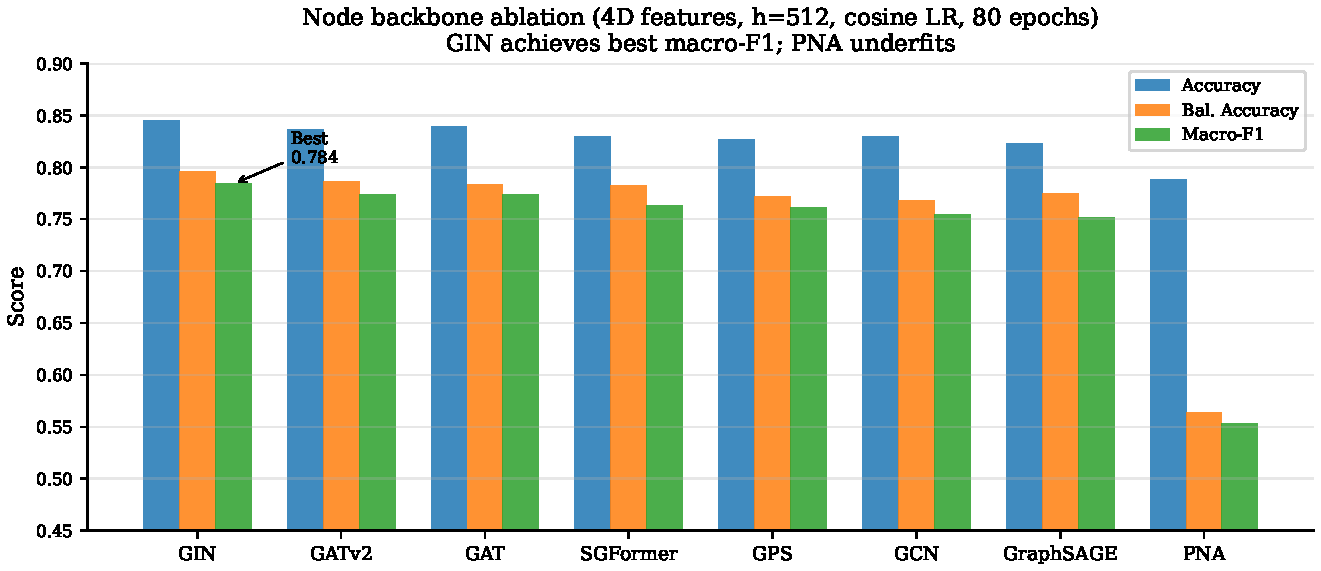
\includegraphics[width=\linewidth]{figures/backbone_ablation.pdf}
  \caption{Node backbone ablation: accuracy, balanced accuracy, and macro-F1
           for eight backbone types (4D features, all other hyperparameters fixed).}
  \label{fig:backbone_ablation}
\end{figure}

\subsection{Per-class Analysis}

The seven hardest classes --- 61, 90, 70, 56, 86, 14, 80 --- contribute
disproportionately to macro-F1 degradation.
Class\,80 achieves near-zero F1 in most configurations due to very few
training examples and high intra-class variability.
Classes 61 and 90 (the near-inseparable pair) produce complementary F1
scores: when the model predicts more class-61 samples correctly it
misclassifies more class-90, and vice versa
(F1 of 0.576 vs.\ 0.850 for the best run).

\subsection{Evaluation Protocol}
\label{sec:eval_protocol}

\paragraph{The 88-class vs.\ 99-class problem.}
The SHREC\,25 test set contains proteins from only \textbf{88 of the 99
families}: 11 families have training samples but zero test samples.
The model still outputs logits for all 99 classes at inference time.

When sklearn's \texttt{f1\_score(..., average='macro')} is called without
an explicit class list it includes every class appearing in the union of
ground-truth and prediction arrays.
Classes absent from the test set have support\,=\,0; their per-class F1 is
set to 0 by \texttt{zero\_division=0}.
The macro average then divides by 99 instead of 88:

\[
  \text{Macro-F1}_{99} = \frac{\sum_{c=0}^{87} F1_c +
    \underbrace{0 + \cdots + 0}_{11}}{99}
  = \frac{88}{99}\;\text{Macro-F1}_{88}
\]

This deflates the reported number by a factor of $88/99 \approx 0.889$
(e.g.\ $0.798 \rightarrow 0.710$ for the 8D model).

\paragraph{How we address it.}
All metrics in this report are computed by passing an explicit class list
to every sklearn metric call:

\begin{verbatim}
labels = sorted(valid_classes)   # 88 class IDs with >=1 test sample
f1_score(y_true, y_pred, average='macro',
         labels=labels, zero_division=0)
\end{verbatim}

This restricts the macro denominator to exactly 88, and classes with no
test samples are excluded from precision, recall, and F1.
Balanced accuracy is computed as macro-averaged recall over the same 88
class list.
Accuracy and weighted-F1 are unaffected (they weight by support, so
zero-support classes contribute nothing regardless).
